\documentclass[12pt]{article}

\usepackage{fullpage}

\usepackage{amsmath,amssymb,amsthm}
\usepackage{graphicx}
\usepackage{color}
\usepackage{algorithm}
\usepackage{algpseudocode}
\usepackage{hyperref}
\hypersetup{
    bookmarks=true,         % show bookmarks bar?
    unicode=false,          % non-Latin characters in Acrobat’s bookmarks
    pdftoolbar=true,        % show Acrobat’s toolbar?
    pdfmenubar=true,        % show Acrobat’s menu?
    pdffitwindow=false,     % window fit to page when opened
    pdfstartview={FitH},    % fits the width of the page to the window
    pdftitle={Computing the Riemann Constant Vector},    % title
    pdfauthor={Swierczewski, Patterson, and Deconinck},     % author
    pdfcreator={Swierczewski},   % creator of the document
    pdfkeywords={mathematics} {algebraic geometry} {riemann constant vector} {theta functions} {abel map} {jacobian},
    pdfnewwindow=true,      % links in new window
    colorlinks=false,       % false: boxed links; true: colored links
    linkcolor=red,          % color of internal links
    citecolor=green,        % color of links to bibliography
    filecolor=magenta,      % color of file links
    urlcolor=cyan           % color of external links
}
\renewcommand{\algorithmicrequire}{\textbf{Input:}\,}
\renewcommand{\algorithmicensure}{\textbf{Output:}}

%
% custom listings (code example) design
%
\usepackage{listings}
\usepackage{upquote}
\newcounter{ipythoncounter}
\setcounter{ipythoncounter}{1}

\renewcommand{\ttdefault}{pcr}
\lstset{
  aboveskip=\bigskipamount,
  belowskip=\bigskipamount,
  basicstyle=\footnotesize\ttfamily,
  language=Python,
  numbers=left,
  stepnumber=9999,
  numberfirstline=true,
  xleftmargin=2cm,
}

\lstnewenvironment{ipythoninput}
                  {
                    \setcounter{lstnumber}{\value{ipythoncounter}}
%                    \renewcommand{\thelstnumber}
%                                 {\bf\ttfamily In [\the\value{lstnumber}]:}
                    \renewcommand{\thelstnumber}
                                 {\bf\ttfamily In [\the\value{ipythoncounter}]:}
                    \lstset{
                      frame=single,
                      frameround=tttt,
                      name=ipythoninput,
                    }
                  }
                  {
                    \addtocounter{ipythoncounter}{1}
                  }

\lstnewenvironment{ipythonoutput}
                  {
                    \addtocounter{ipythoncounter}{-1}
                    \setcounter{lstnumber}{\value{ipythoncounter}}
                    \renewcommand{\thelstnumber}
                                 {\bf\ttfamily Out[\the\value{ipythoncounter}]:}
                    \lstset{
                      name=ipythoninput
                    }
                  }
                  {
                    \addtocounter{ipythoncounter}{1}
                  }

\newtheorem{theorem}{Theorem}
\newtheorem{definition}[theorem]{Definition}

\theoremstyle{definition}
\newtheorem{example}[theorem]{Example}


\DeclareMathOperator{\ZZ}{\mathbb{Z}}
\DeclareMathOperator{\RR}{\mathbb{R}}
\DeclareMathOperator{\CC}{\mathbb{C}}
\DeclareMathOperator{\hg}{\mathfrak{h}_g}
%% \DeclareMathOperator{\dx}{dx}
%% \DeclareMathOperator{\dt}{dt}
\newcommand{\dx}{\,\mathrm{d}x}
\newcommand{\dt}{\,\mathrm{d}t}
\newcommand{\dQ}{\,\mathrm{d}Q}
\DeclareMathOperator{\DivC}{\mathcal{C}}
\DeclareMathOperator{\DivD}{\mathcal{D}}
\DeclareMathOperator{\RCV}{\boldsymbol{K}}
\DeclareMathOperator{\Abel}{\boldsymbol{A}}
\DeclareMathOperator{\HalfLattice}{\Lambda_{1/2}}

\newcommand{\thchar}[2] {\begin{bmatrix}#1\\#2\end{bmatrix}}
\newcommand{\thcharsm}[2] {\left[ \begin{smallmatrix} #1
      \\ #2 \end{smallmatrix} \right]}


\title{Computing the Riemann Constant Vector}
\author{
  \centering
  \footnotesize
  \begin{tabular}{ccc}
    % names
    Bernard Deconinck \footnote{\tt deconinc@uw.edu} &
    Matthew S. Patterson \footnote{\tt matthew.s.patterson@icloud.com} &
    Christopber Swierczewski \footnote{\tt cswiercz@uw.edu} \\
    % address 1
    University of Washington &
    8506 37th Ave SW &
    University of Washington \\
    % address 2
    Department of Applied Mathematics &
    Seattle, WA 98126 &
    Department of Applied Mathematics \\
    % address 3
    Seattle, WA 98195-3925 &
     &
    Seattle, WA 98195-3925
  \end{tabular}
}
\date{\today}

%%%%%%%%%%%%%%%%%%%%%%%%%%%%%%%%%%%%%%%%%%%%%%%%%%%%%%%%%%%%%%%%%%%%%%%%%%%%%%%
\begin{document}
%%%%%%%%%%%%%%%%%%%%%%%%%%%%%%%%%%%%%%%%%%%%%%%%%%%%%%%%%%%%%%%%%%%%%%%%%%%%%%%

\maketitle

\begin{abstract}
The Riemann constant vector is a fundamental ingredient in the study of
Riemann surfaces and their Jacobians. It is necessary to discuss the
Jacobi inversion problem, for the study of the theta divisor, and for
periodic solutions to integrable partial differential equations.

We present a mathematical algorithm and an implementation for computing
the Riemann constant vector on a Riemann surface given by the
desingularization and compactification of a complex plane algebraic
curve. The source code of the implementation is provided in the Python
software package {\sc abelfunctions} \cite{abelfunctions}.
\end{abstract}

%%%%%%%%%%%%%%%%%%%%%%%%%%%%%%%%%%%%%%%%%%%%%%%%%%%%%%%%%%%%%%%%%%%%%%%%%%%%%%%
\section{Introduction}\label{sec:introduction}
%%%%%%%%%%%%%%%%%%%%%%%%%%%%%%%%%%%%%%%%%%%%%%%%%%%%%%%%%%%%%%%%%%%%%%%%%%%%%%%

This paper presents the next step in an ongoing research program to make
effective the calculus on Riemann surfaces represented by complex plane
algebraic curves. Here, ``effective'' means algorithms are devised and
implemented in the form of black-box programs so that different relevant
quantities associated with Riemann surfaces may be computed using a
combination of symbolic and numerical tools in an efficient way. One of
our main objectives in this program is to compute the so-called
finite-genus solutions of integrable partial differential equations,
such as the Korteweg-deVries (KdV), Nonlinear Schr\"odinger (NLS), and
Kadomtsev-Petviashvili (KP) equations. These partial differential
equations have been used extensively for describing a wide variety of
physical phenomena ranging from water waves, nonlinear optics, and
plasma physics to biological applications and cellular automata
\cite{AC91,AS81,DS98,Fordy90}. Other applications are found in convex
optimization and number theory
\cite{Baker97,HeltonVinnikov07,PSV11,PSV12,PocchiolaVegter93}.

As an example, consider the finite-genus solutions $u = u(x,y,t)$ to the
KP equation given by
\begin{equation} \label{eqn:kp}
  u = c + 2 \partial_x^2 \log \theta\Big( \boldsymbol{U}x +
  \boldsymbol{V}y + \boldsymbol{W}t + \Abel\big(P^\infty,\DivD\big) -
  \RCV(P^\infty), \Omega \Big),
\end{equation}
where $c$ is a constant, $\boldsymbol{U}$,$\boldsymbol{V}$, and
$\boldsymbol{W}$ are vectors, and $\theta(z,\Omega)$ denotes the Riemann
theta function parameterized by the Riemann matrix $\Omega$ of Riemann
surface $X$. $\DivD$ is a divisor on $X$, $\Abel(P^\infty,\DivD)$ is its
Abel map with initial place $P^\infty$, and $\RCV(P^\infty)$ is the
Riemann constant vector at $P^\infty$. Details on all of these
components and discussion of the finite-genus solution above are found
in \cite{belokolos,Dubrovin81}. The computation of the Riemann matrix
$\Omega$ is the main topic of \cite{dvh1}. The numerical calculation of
the Riemann theta function is discussed in \cite{DHBvHS03}. Future
papers will present algorithms for computing the remaining quantities
and efficiently computing $u = u(x,y,t)$.

Other approaches exist for computing with Riemann surfaces. Bobenko and
collaborators \cite{belokolos, BobenkoBordag89} compute solutions of
integrable equations using a Schottky group representation for the
associated surface. To our knowledge, the only paper dealing with all
Riemann surfaces represented by algebraic curves is by Frauendiener,
Klein, and Shramchenko who compute the homology of a Riemann surface
from the monodromy of an underlying algebraic curve, following
\cite{dvh1}. Otherwise, authors have restricted themselves to specific
families of Riemann surfaces such as hyperelliptic ones
\cite{FrauendienerKlein06,FrauendienerKlein15} or low genus ones
\cite{DFS97,FinkelSegur85,DeconinckSwierczewski13}. Our aim throughout
is the development of algorithms capable of dealing with arbitrary
compact connected Riemann surfaces, as is required for the investigation
of solutions of, for instance, the KP equation \cite{DS98,Shiota86}.

In this paper we present a mathematical algorithm for computing the
Riemann constant vector (RCV) and a demonstration of an implementation
of this algorithm in {\sc abelfunctions}, an open--source Python
library. The software implementation details, documentation, additional
examples, and installation instructions are found on the project website
\cite{abelfunctions}. The computational examples are presented in the
style of an iPython notebook. The notebook itself can be downloaded from
the project website.




%%%%%%%%%%%%%%%%%%%%%%%%%%%%%%%%%%%%%%%%%%%%%%%%%%%%%%%%%%%%%%%%%%%%%%%%%%%%%%%
\section{Definitions and Background}\label{sec:background}
%%%%%%%%%%%%%%%%%%%%%%%%%%%%%%%%%%%%%%%%%%%%%%%%%%%%%%%%%%%%%%%%%%%%%%%%%%%%%%%

%% %------------------------------------------------------------------------------
%% \subsection{Riemann Surfaces}
%% %------------------------------------------------------------------------------

In this section the required ingredients from the theory of Riemann
surfaces are introduced. Details can be found in the standard references
\cite{FarkasKra92,Springer57} and the review paper \cite{Dubrovin81}. A
computational approach to these topics is found in
\cite{BobenkoKlein11,DeconinckPatterson08} and
\cite{DeconinckPatterson11}.

Let $C$ be a complex plane algebraic curve $C = \{(\alpha,\beta) \in
\CC^2 : f(\alpha,\beta) = 0\}$ where $f \in \CC[x,y]$ is a polynomial
$f(x,y) = \sum_{k=0}^n \alpha_k(x) y^k$ with $\alpha_k \in \CC[x]$. Let
$X$ be the genus $g$ compact and connected Riemann surface obtained by
desingularizing and compactifying the curve $C$; {\it i.e.}, $X$ is a
compact, connected, complex manifold of complex dimension one. Every
compact and connected Riemann surface can be obtained this way
\cite{Griffiths89}.

%% The first homology group $H_1(X,\ZZ)$ of $X$ is the collection of all
%% cycles on $X$ modulo homologous transformations. $H_1(X,\ZZ)$ has a
%% canonical basis of cycles $\{a_1,\ldots,a_g,b_1,\ldots,b_g\}$. The space
%% of holomorphic 1-forms $\Gamma(X,\Omega_X^1)$ on $X$ is the collection
%% of all 1-forms $\omega \in \Omega_X^1$ such that for each local
%% coordinate $z_\alpha : U_\alpha \subset X \to \CC$,
%% \begin{equation}
%%   \omega \big|_{U_\alpha}  = h_\alpha(z_\alpha) dz_\alpha
%% \end{equation}
%% where $h_\alpha : U_\alpha \to \CC$ is a holomorphic
%% function. $\Gamma(X,\Omega_X^1)$ has a basis of holomorphic one-forms
%% $\{\omega_1, \ldots, \omega_g\}$.

Given $X$ of genus $g$ we choose a canonical basis of cycles
$\{a_1,\ldots,a_g,b_1,\ldots,b_g\}$ for the first homology group as well
as a normalized basis of Abelian differentials of the first kind
$\{\omega_1, \ldots, \omega_g\}$. We define the Jacobian $J(X)$ of $X$
using these two ingredients. The {\it period matrix} $[I \; \; \Omega]
\in \CC^{g \times 2g}$ of $X$ is constructed by
\begin{equation} \label{eqn:periodmatrix}
  \oint_{a_j} \omega_i = \delta_{ij}, \qquad
  \oint_{b_j} \omega_i = \Omega_{ij}.
\end{equation}
The matrix $\Omega \in \CC^{g \times g}$ is a {\it Riemann matrix}: a
symmetric complex $g \times g$ matrix with positive definite imaginary
part. The Jacobian is given by the quotient space $J(X) = \CC^g /
\Lambda$ where $\Lambda = \ZZ^g + \Omega \ZZ^g$ is the {\it period
  lattice}.

Algorithms for computing a canonical basis of cycles, a basis of Abelian
differentials of the first kind, and Riemann matrices are given in
\cite{TretkoffTretkoff84}, \cite{Mnuk97,vanHoeij94}, and \cite{dvh1},
respectively. The basis of differentials $\{\tilde{\omega}_1, \ldots,
\tilde{\omega}_g\}$ returned by the algorithm in
\cite{Mnuk97,vanHoeij94} is not necessarily normalized. If a normalized
basis is desired one can be determined by computing the period matrix
$[A \;\; B] \in \CC^{g \times 2g}$ defined by
\begin{equation} \label{eqn:periodmatrixnotnormal}
  \oint_{a_j} \tilde{\omega}_i = A_{ij}, \qquad
  \oint_{b_j} \tilde{\omega}_i = B_{ij}.
\end{equation}
The associated Riemann matrix is constructed by $\Omega = A^{-1}B$ and a
normalized basis of Abelian differentials is determined by
$\boldsymbol{\omega} = A^{-1}\tilde{\boldsymbol{\omega}}$ with
$\tilde{\boldsymbol{\omega}} = [\tilde{\omega}_1, \ldots,
  \tilde{\omega}_g]^T$.


\begin{example} \label{ex:riemannsurface} %%%%%%%%%%%%%%%%%%%%%%%%%%%%%%%%%%%%%
Let $X$ be the Riemann surface obtained via desingularization and
compactification of the non-hyperelliptic, genus 4 curve
\begin{equation}
  C: f(x,y) = x^2y^3 - x^4 + 1 = 0.
\end{equation}
We use this Riemann surface as an example throughout this paper. First
we compute a basis, not necessarily normalized, for the space of Abelian
differentials of the first kind.
\begin{ipythoninput}
from sympy.abc import x,y
from abelfunctions import (RiemannSurface, RiemannTheta, Jacobian,
                           AbelMap, RiemannConstantVector, puiseux)

f = x**2*y**3 - x**4 + 1
X = RiemannSurface(f,x,y)
g = X.genus()

omega = X.holomorphic_differentials()
print 'differentials:'
for omegai in omega:
    print omegai
print 'genus:', g
\end{ipythoninput}
\begin{ipythonoutput}
differentials:
1/(3*x**2*y**2)
x/(3*x**2*y**2)
x*y/(3*x**2*y**2)
x**2/(3*x**2*y**2)
genus: 4
\end{ipythonoutput}
Next, we compute a canonical basis of cycles on $X$. We plot the
projection of the cycle $a_1$ in the complex $x$- and $y$-planes,
respectively.
\begin{ipythoninput}
a = X.a_cycles()
b = X.b_cycles()

# use 256 points to plot the x- and y-parts of the path
a[0].plot_x(256, color='blue', linewidth=2, linestyle='dashed')
a[0].plot_y(256, color='green', linewidth=2)
\end{ipythoninput}
\vspace{-12pt}
\begin{ipythonoutput}
\end{ipythonoutput}
\hspace{2pt} {\footnotesize\bf\ttfamily Out[2]:}

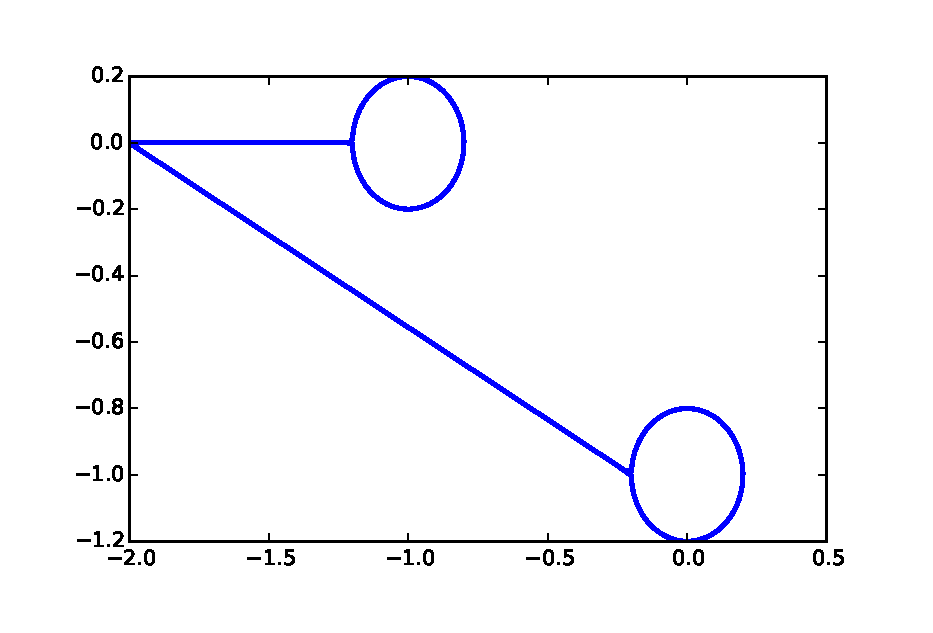
\includegraphics[width=0.45\textwidth]{a1x.eps}
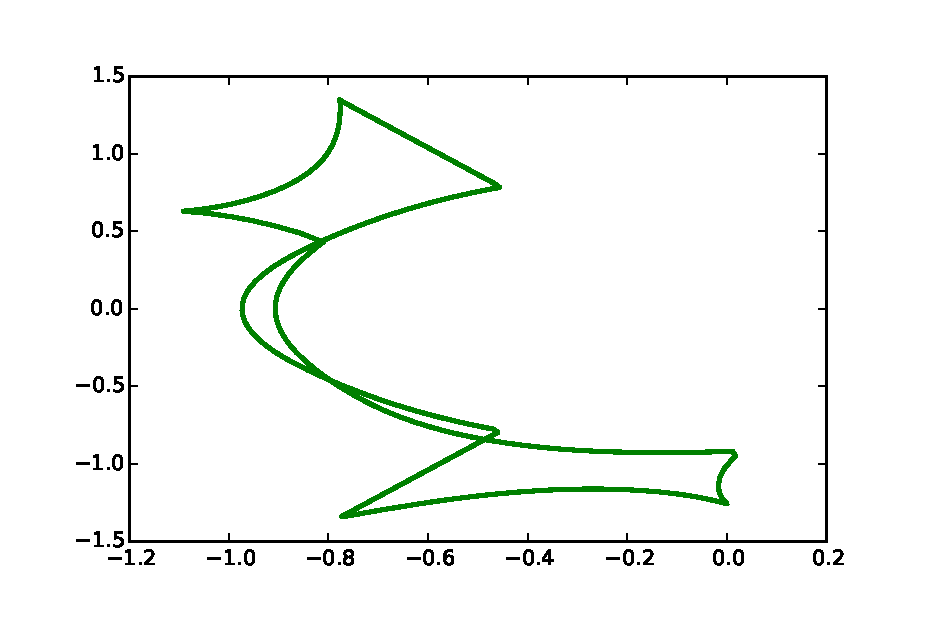
\includegraphics[width=0.45\textwidth]{a1y.eps}

Finally, we compute the associated Riemann matrix by numerically
integrating the non-normalized basis of holomorphic differentials around
the $a$- and $b$-cycles and computing $\Omega = A^{-1}B$. By default,
{\sc abelfunctions} numerically integrates differentials along Riemann
surface paths using a tolerance of $10^{-8}$. We verify that $\Omega$ is
symmetric and has positive definite imaginary part by computing
$||\Omega-\Omega^T||_2$ and the eigenvalues of $\text{Im}(\Omega)$.
\begin{ipythoninput}
# for brevity, we only print the first four significant digits
import numpy
numpy.set_printoptions(precision=4, suppress=True)

tau = X.period_matrix()
A = tau[:g,:g]
B = tau[:g,g:]
Omega = X.riemann_matrix()  # returns A**(-1)*B

print A
print B
print Omega
\end{ipythoninput}
\begin{ipythonoutput}
[[ 0.2800+1.045j   0.2800-0.485j  -1.8100+1.045j   0.0000-0.j    ]
 [ 0.6625-1.1475j  0.6625+0.3825j -0.6625-1.1475j -0.0000+1.53j  ]
 [-0.8347+0.4819j -0.8347+0.4819j  0.8347-1.4457j  0.0000+1.9276j]
 [-1.0450+0.28j   -1.0450+1.81j   -0.4850+0.28j    0.0000+0.j    ]]

[[-0.2800+0.485j   0.2800-1.045j   0.0000-2.09j    0.7650-1.325j ]
 [ 0.6625+0.3825j -0.6625+0.3825j  0.0000-0.765j   0.0000-1.53j  ]
 [-0.8347+0.4819j  0.8347-1.4457j  0.0000-0.9638j -1.6694-0.9638j]
 [ 1.0450-1.81j   -1.0450-0.28j   -0.0000-0.56j    0.7650-1.325j ]]

[[ 0.3934+0.795j  -0.7541-0.3691j -0.4426-0.0284j  0.2049+0.2697j]
 [-0.7541-0.3691j  0.2787+0.8518j  0.0984+0.1988j -0.4344-0.1562j]
 [-0.4426-0.0284j  0.0984+0.1988j -0.3770+0.6815j -0.9180+0.4543j]
 [ 0.2049+0.2697j -0.4344-0.1562j -0.9180+0.4543j -1.2787+0.8802j]]
\end{ipythonoutput}
\begin{ipythoninput}
symmetric_error = numpy.linalg.norm(Omega - Omega.T)
imag_part_evals = numpy.linalg.eigvals(Omega.imag)

print 'error:', symmetric_error
print 'evals:', imag_part_evals
\end{ipythoninput}
\begin{ipythonoutput}
error: 3.54420889595e-10
evals: [ 1.4038  1.1654  0.4294  0.21  ]
\end{ipythonoutput}
\end{example}




%------------------------------------------------------------------------------
\subsection{Places and Divisors}
%------------------------------------------------------------------------------


\begin{definition}\label{def:puiseux}
Given a place $P \in X$, a local representation of the Riemann surface
centered at $P$ is given using a Puiseux series
\begin{align} \label{eqn:puiseux}
  P =
  \begin{cases}
    x_P(t) = \alpha + \lambda t^e, \\
    y_P(t) = \sum_{k=0}^\infty \beta_k t^{n_k},
  \end{cases}
\end{align}
where $\alpha, \lambda, \beta_k \in \CC$, and $e, n_k \in \ZZ$
\cite{bliss}.
\end{definition}
\noindent Places lie ``above'' the curve $C$ in the sense that
evaluating $P = (x_P(t), y_P(t))$ at $t=0$ maps the place $P$ onto a
point $(\alpha,\beta)$ of the curve.

Let $R(f,\partial_y f)(x)$ be the resultant of $f(x,y)$ and $\partial_y
f(x,y)$ with respect to $y$ \cite{Griffiths89}. The roots $\alpha \in
\CC$ of $R$ correspond to the {\it discriminant points} of $C$, which
consist of the branch points and singular points of the curve. A place
is called {\it discriminant} if it lies above a discriminant point of
$C$. Otherwise, it is {\it regular}. An algorithm for computing Puiseux
series expansions is found in \cite{Duval89} and
\cite{PoteauxRybowicz08}.


\begin{example} \label{ex:places} %%%%%%%%%%%%%%%%%%%%%%%%%%%%%%%%%%%%%%%%%%%%%
Continuing from Example \ref{ex:riemannsurface}, there is one place on
$X$ lying above the discriminant point $x=0$:
\begin{equation}
  P =
  \begin{cases}
    x_{P}(t) &= -t^3, \\
    y_{P}(t) &= -t^{-2} + O\left( t^2 \right).
  \end{cases}
\end{equation}
Let $\alpha_1$, $\alpha_2$, and $\alpha_3$ denote the roots of the
polynomial $f(2,y) = 4y^3 - 15$. There are three regular places
$P_1$,$P_2$, and $P_3$ lying above $x=2$:
\begin{equation}
  P_i =
  \begin{cases}
    x_{P_i}(t) &= 2 + t, \\
    y_{P_i}(t) &= \alpha_i + \tfrac{17}{45}\alpha_i t + O\left(t^2\right),
  \end{cases}
\end{equation}
We confirm the form of these places computationally.
\begin{ipythoninput}
places_above_zero = X(0)
print places_above_zero
\end{ipythoninput}
\begin{ipythonoutput}
[(-t**3, -1/t**2 + O(t**2))]
\end{ipythonoutput}
By default, {\sc abelfunctions} does not determine the Puiseux series
expansions of regular places since each regular place above a given
$x=\alpha$ maps to a unique point $(\alpha,\beta) \in C$. We can request
these series expansions using the {\tt puiseux()} function.
\begin{ipythoninput}
print 'Places:'
places_above_two = X(2)
for P in places_above_two:
    print P

print 'Puiseux:'
series_at_two = puiseux(f,x,y,2)
for p in series_at_two:
    print p
\end{ipythoninput}
\begin{ipythonoutput}
Places:
(2, RootOf(4*_y**3 - 15, 0))
(2, RootOf(4*_y**3 - 15, 1))
(2, RootOf(4*_y**3 - 15, 2))

Puiseux:
(t + 2, RootOf(4*_y**3 - 15, 0) + 17*t*RootOf(4*_y**3 - 15, 0)/45 + O(t**2))
(t + 2, RootOf(4*_y**3 - 15, 1) + 17*t*RootOf(4*_y**3 - 15, 1)/45 + O(t**2))
(t + 2, RootOf(4*_y**3 - 15, 2) + 17*t*RootOf(4*_y**3 - 15, 2)/45 + O(t**2))
\end{ipythonoutput}

\end{example}

Related to places is the notion of a divisor
\cite{Griffiths89,Springer57}.
\begin{definition} \label{def:divisor}
A divisor $\DivD$ on the Riemann surface $X$ is a finite formal linear
combination of places $P_i$ with multiplicities $n_i$:
\begin{equation}
\DivD = \sum_i n_i P_i.
\end{equation}
The sum
\begin{equation}
\deg \DivD = \sum_i n_i
\end{equation}
is called the degree of $\DivD$.
\end{definition}
The set of all divisors on a Riemann surface forms an Abelian group
$\text{Div}(X)$ under addition. A divisor with all $n_i \geq 0$ is
called {\it positive} or {\it effective}. A {\it valuation divisor},
important for the calculation of the Riemann constant vector, is
obtained by examining the root and pole structure of a meromorphic
one-form on $X$.
\begin{definition} \label{def:valuationdivisor}
Let $\Omega_X^1$ denote the set of meromorphic one-forms on $X$ and let
$\nu \in \Omega_X^1$ have $m$ zeros of multiplicity $p_j$ at the places
$P_j$ and $n$ poles of multiplicity $q_j$ at the places $Q_j$. Then
\begin{equation} \label{eqn: valuation divisor}
  (\nu)_\text{val} = \sum_{i=1}^m p_iP_i - \sum_{j=1}^n q_jQ_j
\end{equation}
is called the valuation divisor of $\nu$. A divisor $\DivC \in
\text{Div}(X)$ is called {\it canonical} if $\DivC = (\nu)_\text{val}$
for some $\nu \in \Omega_X^1$.
\end{definition}
All canonical divisors have the same degree and, by the Riemann--Roch
Theorem, this degree is $\deg \DivC = 2g - 2$ \cite{Springer57}. Note
that every Abelian differential of the first kind is trivially
meromorphic, since it is a holomorphic one-form, and its valuation
divisor has $q_j = 0$ for all $j$. Consequently, every such differential
has exactly $2g-2$ zeros including multiplicities.


\begin{example} \label{ex:divisors} %%%%%%%%%%%%%%%%%%%%%%%%%%%%%%%%%%%%%%%%%%%
We use the places computed in Example \ref{ex:places} to construct
divisors on the Riemann surface $X$.
\begin{ipythoninput}
P = places_above_zero[0]
Q = places_above_two[0]
D = 3*P + Q
print 'Divisor:', D
print 'Degree:', D.degree
\end{ipythoninput}
\begin{ipythonoutput}
Divisor: 3(-t**3, -1/t**2 + O(t**2)) + (2, RootOf(4*_y**3 - 15, 0))
Degree: 4
\end{ipythonoutput}
\end{example}


%------------------------------------------------------------------------------
\subsection{The Abel Map}
%------------------------------------------------------------------------------

\begin{definition}\label{def:abelmap}
  Let $P \in X$ be a fixed place. The Abel Map $\boldsymbol{A} : X \to
  J(X)$ is defined by
  \begin{equation} \label{eqn:abel1}
    \boldsymbol{A}(P,Q) = \big( A_1(P,Q), \ldots, A_g(P,Q) \big),
  \end{equation}
  where
  \begin{equation} \label{eqn:abel2}
    A_j(P,Q) = \int_P^Q \omega_j,
  \end{equation}
  and the path chosen from $P$ to $Q$ is the same for each $A_j$. The
  Abel map is written in vector form as
  \begin{equation} \label{eqn:abel-vector}
    \boldsymbol{A}(P,Q) = \int_P^Q \boldsymbol{\omega}.
  \end{equation}
\end{definition}
The definition of the Abel map can be extended to divisors: let $\DivD =
\sum_i n_i P_i$. We define
\begin{equation} \label{eqn:abel-divisors}
  \boldsymbol{A}(P,\DivD) = \sum_i n_i \boldsymbol{A}(P,P_i).
\end{equation}
The Abel Map is independent of the path $\gamma$ from $P$ to $Q$ chosen
on $X$ for if $\gamma$ and $\eta$ are two such paths then their
difference is a linear combination of homology basis cycles. The
integral of $\boldsymbol{\omega}$ along this closed path is a lattice
element and therefore is congruent to zero in $J(X)$.

An algorithm for computing the Abel map is described in
\cite{DeconinckPatterson11}. The implementation in {\sc abelfunctions}
is based on this algorithm.

\begin{example}
{\sc abelfunctions} selects a regular ``base place'' $P_0$ from which to
construct all paths on $X$. When given a single argument {\tt AbelMap()}
returns $\Abel(P_0,P)$.
\begin{ipythoninput}
J = Jacobian(X)   # reduces vectors modulo lattice ZZ^g + Omega ZZ^g
z1 = AbelMap(P)   # Abel map from P0 to P
z2 = AbelMap(Q)   # Abel map from P0 to Q
z3 = AbelMap(P,Q) # Abel map from P to Q
print z1
print z2
print z3

# numerically verify that A(P,Q) = A(P0,Q) - A(P0,P)
print numpy.linalg.norm( J((z2-z1) - z3) )
\end{ipythoninput}
\begin{ipythonoutput}
[[-0.5261+0.0864j  0.0669+0.6392j -0.7495+1.1037j -1.5030+1.0356j]]
[[-0.3875+0.1157j -0.0290+0.4437j -0.4532+0.7774j -0.9721+0.6732j]]
[[ 0.1468-0.0985j  0.8467+0.6989j  0.0996+1.0083j -1.1003+0.8159j]]
3.80631643473e-16
\end{ipythonoutput}
The Abel map accepts divisors as well.
\begin{ipythoninput}
w = AbelMap(D)
print w

# verify that w = 3*z1 + z2 mod period lattice
z = J(3*z1 + z2)
print numpy.linalg.norm(w-z)
\end{ipythoninput}
\begin{ipythonoutput}
[[ 0.0670-0.1361j  0.9421+0.7429j -0.4887+0.7663j -1.5057+0.6992j]]
1.57107346e-15
\end{ipythonoutput}
\end{example}



%------------------------------------------------------------------------------
\subsection{The Riemann Constant Vector}
%------------------------------------------------------------------------------

\begin{definition} \label{def:rcv}
Let $X$ be a genus $g$ Riemann surface with associated Riemann matrix
$\Omega$. The Riemann constant vector $\RCV : X \to J(X)$ is defined as
\begin{equation} \label{eqn:rcv1}
  \RCV(P) = \big( K_1(P), \ldots, K_g(P) \big),
\end{equation}
where
\begin{equation} \label{eqn:rcv2}
  K_j(P) = \frac{1 + \Omega_{jj}}{2} - \sum_{k \neq j}^g
           \oint_{a_k} \omega_k(Q) A_j(P,Q).
\end{equation}
\end{definition}
Once we know the value of $\RCV(P_0)$ the value of $\RCV(P)$ is
determined using only a shift by the Abel map:
\begin{theorem} \label{thm:RCVshift}
  Let $P_0,P$ be places on a genus $g$ Riemann surface $X$. Then
  \begin{equation} \label{eqn:RCVshift}
    \RCV(P) = \RCV(P_0) + (g-1)\Abel(P_0,P).
  \end{equation}
\end{theorem}
\begin{proof}
Let $Q$ be an arbitrary place on $X$. By the definition of the Abel map,
$\Abel(P,Q) = \Abel(P,P_0) + \Abel(P_0,Q)$. Using this identity in the
definition of the RCV we obtain
\begin{align} \label{eqn:RCVshift1}
  K_j(P)
  &=
  \frac{1 + \Omega_{jj}}{2}
  -
  \sum_{k \neq j}^g
  \oint_{a_k} \omega_k(Q) A_j(P,Q) \dQ  \notag \\
  &=
  \frac{1 + \Omega_{jj}}{2}
  -
  \sum_{k \neq j}^g
  \oint_{a_k} \omega_k(Q) \Big( A_j(P,P_0) + A_j(P_0,Q) \Big) \dQ  \notag \\
  &=
  \frac{1 + \Omega_{jj}}{2}
  -
  \sum_{k \neq j}^g
  \oint_{a_k} \omega_k(Q) A_j(P,P_0) \dQ
  -
  \sum_{k \neq j}^g
  \oint_{a_k} \omega_k(Q) A_j(P_0,Q) \dQ.
\end{align}
The $j$th-component of the Abel map appearing in the first sum has no
dependence on the variable of integration $Q$ nor on the summation index
$k$. Therefore,
\begin{align} \label{eqn:RCVshift2}
  K_j(P)
  &=
  \frac{1 + \Omega_{jj}}{2}
  -
  A_j(P,P_0)
  \sum_{k \neq j}^g
  \oint_{a_k} \omega_k(Q) \dQ
  -
  \sum_{k \neq j}^g
  \oint_{a_k} \omega_k(Q) A_j(P_0,Q) \dQ \notag \\
  &=
  \frac{1 + \Omega_{jj}}{2}
  -
  A_j(P,P_0) (g-1)
  -
  \sum_{k \neq j}^g
  \oint_{a_k} \omega_k(Q) A_j(P_0,Q) \dQ \notag \\
  &=
  K_j(P_0) + (g-1)A_j(P_0,P).
\end{align}
\end{proof}
The primary computational benefit to using the result of Theorem
\ref{thm:RCVshift} is that most of the work in evaluating $\RCV$ comes
from evaluating it at a fixed place $P_0$. Once this is done, we only
need the Abel map to determine $\RCV$ for all other places $P \in X$. In
{\sc abelfunctions} a fixed place of the Riemann surface is
automatically chosen.

The inspiration behind the algorithm for computing the RCV described in
the following section comes from the following two theorems. Theorem
\ref{thm:rcvequiv} characterizes a certain class of divisors in terms of
the RCV, a proof of which is found in \cite{FarkasKra92}.
\begin{theorem} \label{thm:rcvequiv}
  Let $\DivC$ be a divisor on a genus $g$ Riemann surface $X$ of degree
  $2g - 2$. Then $\DivC$ is a canonical divisor if and only if
  \begin{equation} \label{eqn:rcvequiv}
    2\RCV(P) \equiv -\Abel(P,\DivC).
  \end{equation}
\end{theorem}
\noindent Theorem \ref{thm:thetadivisor} establishes a connection
between the Riemann theta function and the RCV, a proof of which is also
found in \cite{FarkasKra92}.
\begin{definition} \label{def:riemanntheta}
  The Riemann theta function $\theta: J(X) \times \hg \to \CC$ is
  defined by
  \begin{equation} \label{eqn:riemanntheta}
    \theta(z,\Omega)
    =
    \sum_{n \in \ZZ^g}
    e^{2 \pi i \left( \tfrac{1}{2} n \cdot \Omega n + n \cdot z \right)}.
  \end{equation}
  This series converges absolutely and uniformly on compact sets in
  $J(X) \times \hg$ where $\hg$ is the space of all Riemann matrices.
\end{definition}

\begin{theorem} \label{thm:thetadivisor}
  Let $\Omega$ be the Riemann matrix associated with the Riemann surface
  $X$ and $P_0 \in X$ an arbitrary place. Then a vector $\boldsymbol{W}
  \in J(X)$ satisfies
  \begin{equation} \label{eqn:thetadivisor1}
    \theta(\boldsymbol{W}, \Omega) = 0,
  \end{equation}
  if and only if there exists a divisor $\DivD = P_1 + \cdots P_{g-1}$
  such that
  \begin{equation} \label{eqn:thetadivisor2}
    \boldsymbol{W} = \boldsymbol{A}(P_0, \DivD) + \boldsymbol{K}(P_0).
  \end{equation}
\end{theorem}
Note that $\DivD$ may contain a place of multiplicity greater than
one. The primary requirement of $\DivD$ is that it is of degree $g-1$
and is effective. The set $\Theta := \{ \boldsymbol{W} \in J(X) :
\theta(\boldsymbol{W},\Omega) = 0\}$ is known as the {\it theta divisor}
of the Riemann surface $X$. It is a $(g-1)$ complex--dimensional
subvariety of $J(X)$. Theorem \ref{thm:thetadivisor} states that $\Theta
= \Abel\left(P_0,SX^{g-1}\right) + \boldsymbol{K}(P_0)$ where $SX^{g-1}$
is the $(g-1)$--fold symmetric product of the Riemann surface.




%%%%%%%%%%%%%%%%%%%%%%%%%%%%%%%%%%%%%%%%%%%%%%%%%%%%%%%%%%%%%%%%%%%%%%%%%%%%%%%
\section{Computing the Riemann Constant Vector}
%%%%%%%%%%%%%%%%%%%%%%%%%%%%%%%%%%%%%%%%%%%%%%%%%%%%%%%%%%%%%%%%%%%%%%%%%%%%%%%





In this section we present an algorithm for computing the Riemann
constant vector as well as a demonstration of its implementation in {\sc
  abelfunctions}. First we present an overview of and the motivation
behind the algorithm. We describe the two primary components of the
algorithm later in this section.

Theorem \ref{thm:rcvequiv} suggests an approach to computing the RCV
provided we can compute a canonical divisor of the Riemann
surface. However, even with such a divisor the theorem only makes a
statement about the value of $2\RCV(P_0)$. That is, one would like to
say
\begin{equation}
\RCV(P_0) \equiv - \tfrac{1}{2} \Abel(P_0,\DivC),
\end{equation}
but division is not unique in this equivalence class. In general, there
are $2^{2g}$ {\it half-lattice vectors} $\boldsymbol{h} \in
\tfrac{1}{2}\Lambda$ such that $\RCV(P_0) \equiv \boldsymbol{h} -
\tfrac{1}{2}\Abel(P_0,\DivC)$. Therefore, a second objective is to find
an appropriate half-lattice vector.

\begin{algorithm}[H]
\caption{\tt riemann\_constant\_vector}
\label{alg:rcv}
\begin{algorithmic}[1]
  \Require Riemann surface $X$ given by the desingularization and
  compactification of complex plane algebraic curve $C : f(x,y) = 0$

  \Require place $P \in X$

  \Ensure Riemann constant vector $\RCV(P)$

  \State compute the Riemann matrix $\Omega$

  \State $\DivC \gets$ \verb=canonical_divisor()=
  \Comment{Algorithm \ref{alg:canonical}}

  \State $\boldsymbol{h} \gets$ \verb=half_lattice_vector()=
  \Comment{Algorithm \ref{alg:half-lattice-vector}}

  \State $\RCV_0 \gets \boldsymbol{h} - \tfrac{1}{2}\Abel(P_0,\DivC)
  \bmod{\Lambda}$

  \State $\RCV \gets \RCV_0 + (g-1)\Abel(P_0,P)$

  \State \Return $\RCV$
\end{algorithmic}
\end{algorithm}

The rest of this section presents in detail the subroutines
\verb=canonical_divisor= and \verb=half_lattice_vector= which provide
the necessary remaining ingredients for the above algorithm.



%------------------------------------------------------------------------------
\subsection{Computing a Canonical Divisor}\label{sec:canonical}
%------------------------------------------------------------------------------



Determining the zeros and poles of a meromorphic one-form
\begin{equation} \label{eqn:meromorphic-one-form}
\nu = \frac{p(x,y)}{q(x,y)}\dx
\end{equation}
is not as straightforward as finding the roots of the polynomials $p$
and $q$. One challenge comes from analyzing the local behavior of
$\dx$. Furthermore, it may occur that the numerator and denominator have
the same order of vanishing at some place $P \in X$ in which case $P$ is
neither a root nor pole of $\nu$.

Let $P \in X$ be a place with Puiseux series representation $(x_P(t),
y_P(t))$ where $t$ is a local parameter as given in Definition
\ref{def:puiseux}. A necessary condition for $P$ to be a root or pole of
$\nu$ is that
\begin{equation}
  p\big(x_P(t), y_P(t)\big) \Big|_{t=0} \! = 0,
  \qquad
  q\big(x_P(t), y_P(t)\big) \Big|_{t=0} \! = 0,
  \qquad \text{or} \qquad
  \frac{\dx_P}{\dt}\big(0\big) = 0.
\end{equation}
In particular, to determine if $P \in (\nu)_\text{val}$ we substitute
the Puiseux series representation into $\nu$ and expand as a Laurent
series in $t$:
\begin{align} \label{eqn:localization}
\nu \Big|_P
&=
\frac{p\big(x_P(t),y_P(t)\big)}{q\big(x_P(t),y_P(t)\big)} \dx_P(t) \notag \\
&=
\frac{p(t)}{q(t)} x_P'(t) \dt \notag \\
&=
\Big( c t^{\text{val}(\nu,P)} + \cdots \Big) \dt,
\end{align}
where $\text{val}(\nu,P)$ is the leading order behavior of $\nu$ at
$P$. This gives us a test for determining if $P$ is a member of the set
of places appearing in $(\nu)_\text{val}$: if $\text{val}(\nu,P) < 0$
then $P$ is a pole, if $\text{val}(\nu,P) > 0$ then $P$ is a zero,
otherwise $P$ does not appear in the valuation divisor of $\nu$. The
multiplicity of the zero or pole is equal to $|\text{val}(\nu,P)|$.

With the above membership test what remains is to construct a set of
places $\mathcal{P}_\nu$ guaranteed to contain the places appearing in
$(\nu)_\text{val}$. We obtain the valuation divisor by applying the
membership test to each $P \in \mathcal{P}_\nu$. Consider the resultant
$R(f,p)(x)$ of $f$ and $p$ with respect to $y$. By definition, the roots
of $R$ are the points $\alpha \in \CC$ such that
\begin{equation}
f(\alpha,y) = 0 \quad \text{and} \quad p(\alpha, y) = 0
\end{equation}
have simultaneous solutions. Therefore, for a place $P$ to be a zero of
$p$ it must be the case that the $x$-projection of $P$, $x_P(0)$, is a
root of the resultant $R$. Similarly, for $P$ to be a zero of $q$ its
$x$-projection $x_P(0)$ must be a root of the resultant $R(f,q)(x)$. We
also need to include the places $P$ which cause $\dx$ to vanish. This
occurs when $(\dx_P/\dt)(0) = x'_P(0) = 0$. That is, when $P$ lies above
a branch point of $f$.

Define the sets
\begin{align}
  \mathcal{X}_\nu^{(1)}
  &=
  \left\{
  \alpha \in \CC \; | \; R(f,p)(\alpha) = 0
  \right\}, \notag \\
  \mathcal{X}_\nu^{(2)}
  &=
  \left\{
  \alpha \in \CC \; | \; R(f,q)(\alpha) = 0
  \right\}, \notag \\
  \text{and} \quad \mathcal{X}_\nu^{(3)}
  &=
  \left\{ \alpha \in \CC \; | \; \alpha \text{ is
    a branch point of $f$} \right\}.
\end{align}
Since the representation of the one-form in
\eqref{eqn:meromorphic-one-form} only captures its affine behavior it is
necessary to examine its behavior at all places lying above
$x=\infty$. Define
\begin{equation}
\mathcal{X}_\nu
=
\mathcal{X}_\nu^{(1)} \cup
\mathcal{X}_\nu^{(2)} \cup
\mathcal{X}_\nu^{(3)} \cup
\{ \infty \}.
\end{equation}
This consists of all $x$-points above which there may be a place $P$
where $\nu$ vanishes. That is, the only places we need to check are
those with $x$-projections in $\mathcal{X}_\nu$. Therefore, the set
\begin{equation}
\mathcal{P}_\nu =
\left\{ P \in X \; | \; x_P(0) \in \mathcal{X}_\nu
\right\},
\end{equation}
is guaranteed to contain the places appearing in $(\nu)_\text{val}$. The
Puiseux algorithm is well-designed to compute this set.

This procedure is simplified when computing the valuation divisor of an
Abelian differential of the first kind. Recall that every such
differential is trivially a meromorphic one-form and therefore can be
used to compute a canonical divisor. We could use one of the normalized
basis elements $\{\omega_1, \ldots, \omega_g\}$ to obtain a canonical
divisor on $X$ but it is preferred to use the non-normalized
differentials $\{\tilde{\omega}_1, \ldots, \tilde{\omega}_g\}$ returned
by {\sc abelfunctions}. This is done for several performance-related
reasons:
\begin{itemize}
\item We already compute these differentials for the purposes of
  determining the period matrix of $X$ as well as in defining the Abel
  map.
\item Fewer resolvent sets need to be determined. The denominator of
  every Abelian differential of the first kind is $\partial_y f(x,y)$
  \cite{Brieskorn86,Noether83} so one can compute the resolvent set of
  $f$ with $\partial_y f$ once and use the results for any given basis
  element $\tilde{\omega} = \tilde{\omega}_i$. This particular resolvent
  set consists of the discriminant points of $f$ and is already used in
  the period matrix calculations.
\item The non-normalized differentials usually have simple, often
  monomial, numerators making the set
  $\mathcal{X}_{\tilde{\omega}}^{(1)}$ easier to compute and have
  smaller cardinality.
\item The set of $P$ such that $x_P(0)$ is a branch point of $f$ is
  contained in the set of discriminant points of $f$. Therefore, the
  computation of the set $\mathcal{X}_{\tilde{\omega}}^{(3)}$ is a
  redundant calculation and is omitted.
\item In general, the valuation divisors of Abelian differentials of the
  first kind consist of fewer distinct places. The degree of every
  canonical divisor is $2g-2$. Therefore, there must always be $2g-2$
  more zeros than poles, counting multiplicities. Since Abelian
  differentials of the first kind have no poles, no negative degree
  places appear in the valuation divisor thus minimizing the total
  number of places to check.
\item Algorithm \ref{alg:canonical} iteratively checks each $P \in
  \mathcal{P}_{\tilde{\omega}}$ for membership in the set of places in
  $\DivC = (\tilde{\omega})_\text{val}$. By using Abelian differentials
  of the first kind we can terminate this procedure the moment $\deg
  \DivC$ reaches $2g-2$ since each $P\in\mathcal{P}_{\tilde{\omega}}$
  contributes a non-negative amount to the degree. For this reason, we
  distinguish between the set of $\mathcal{X}_{\tilde{\omega}}$ and
  corresponding places $\mathcal{P}_{\tilde{\omega}}$ in order to avoid
  unnecessarily computing Puiseux series expansions.
\end{itemize}

An algorithm for computing the valuation divisor of an Abelian
differential of the first kind is given below.
\begin{algorithm}[H]
\caption{{\tt canonical\_divisor} - canonical divisor of a Riemann surface}
\label{alg:canonical}
\begin{algorithmic}[1]
  \Require Riemann surface $X$ given by the desingularization and
  compactification of complex plane algebraic curve $C : f(x,y) = 0$

  \Require an Abelian differential of the first kind $\tilde{\omega} =
  p(x,y) / \partial_y f(x,y) \dx$ on $X$

  \Ensure canonical divisor $\DivC = (\tilde{\omega})_\text{val}$

  \State $\DivC \gets$ zero divisor

  \State $\mathcal{X}_{\tilde{\omega}}^{(1)} \gets$ roots of resolvent
  $R(f,p)(x) = 0$

  \State $\mathcal{X}_{\tilde{\omega}}^{(2)} \gets$ discriminant points of $f$

  \State $\mathcal{X}_{\tilde{\omega}} \gets
  \mathcal{X}_{\tilde{\omega}}^{(1)} \cup
  \mathcal{X}_{\tilde{\omega}}^{(2)} \cup \{ \infty \}$

  \For{$\alpha \in \mathcal{X}_{\tilde{\omega}}$}

  \State $\mathcal{P}_{\tilde{\omega}}^\alpha \gets \left\{ P \in X \; |
  \; x_P(0) = \alpha \right\}$

  \For{$P \in \mathcal{P}_{\tilde{\omega}}^\alpha$}

  \State $n \gets \text{val}\left(\tilde{\omega},P\right)$

  \State $\DivC \gets \DivC + \,n P$

  \If{$\deg \DivC = 2g - 2$}
  \State \Return $\DivC$
  \EndIf

  \EndFor

  \EndFor

  \State {\bf raise error}(``Not enough places found.'')

\end{algorithmic}
\end{algorithm}
Some notes about the algorithm:
\begin{itemize}
\item Only the leading order behavior of the Puiseux series of each
  place $P \in \mathcal{P}_\omega^\alpha$ determining
  $\text{val}(\tilde{\omega},P)$ is needed implying that computing only
  the ``singular part'' of these expansions using the method of Duval is
  sufficient \cite{Duval89}.
\item Since any Abelian differential of the first kind is sufficient for
  computing a canonical divisor we can choose the basis element
  $\tilde{\omega}_i$ with lowest total degree numerator $p=p(x,y)$ to
  reduce the number of places to check and amount of symbolic arithmetic
  to perform.
\item Algorithm \ref{alg:canonical} terminates once the target degree is
  met and will spend no further effort computing places and
  valuations. Since the numerators of $\tilde{\omega}_i$ are often
  monomial, a significant gain in efficiency is observed when
  $\mathcal{X}_{\tilde{\omega}}$ is ordered such that places over $x \in
  \{0,\infty\}$ are checked first. For testing purposes, the algorithm
  can be modified to verify that $\text{val}(\tilde{\omega},P) = 0$ for
  all remaining $P \in \mathcal{P}_{\tilde{\omega}}$ after the degree
  requirement is met.
\item If the main loop in Algorithm \ref{alg:canonical} terminates
  before the requisite degree is achieved then an error is
  reported. This is included as an additional check for the
  algorithm. Yet another test is to verify that $\deg
  (\tilde{\omega}_i)_\text{val} = 2g-2$ for all basis elements
  $\tilde{\omega}_i$. Because this is an expensive calculation it is not
  performed by default. Instead it is relegated to the {\sc
    abelfunctions} test suite.
\end{itemize}

\begin{example} \label{ex:canonical} %%%%%%%%%%%%%%%%%%%%%%%%%%%%%%%%%%%%%%%%%%
For each non-normalized Abelian differential of the first kind from
Example~\ref{ex:riemannsurface},
\begin{equation}
  \tilde{\omega}_1 = \frac{\dx}{3x^2y^2}, \quad
  \tilde{\omega}_2 = \frac{x\dx}{3x^2y^2}, \quad
  \tilde{\omega}_3 = \frac{xy\dx}{3x^2y^2}, \quad
  \tilde{\omega}_4 = \frac{x^2\dx}{3x^2y^2},
\end{equation}
we compute its corresponding canonical divisor. First, we verify that
\begin{equation}
  (\tilde{\omega}_1)_\text{val} = 6 P_{x=\infty}
  \qquad
  \text{where}
  \qquad
  P_{x=\infty} = \left( t^{-3}, t^{-2} + O\left( t^2 \right) \right).
\end{equation}
That is, the valuation divisor consists of the single place,
$P_{x=\infty}$, of multiplicity six.
\begin{ipythoninput}
C0 = omega[0].valuation_divisor()
for place,multiplicity in C0:
    print multiplicity, place
print 'Degree:', C0.degree
\end{ipythoninput}
\begin{ipythonoutput}
6 (t**(-3), t**(-2) + O(t**2))
Degree: 6
\end{ipythonoutput}
On the other hand, $(\tilde{\omega}_2)_\text{val}$ consists of two
distinct places each of multiplicity three:
\begin{equation}
  (\tilde{\omega}_2)_\text{val} = 3 P_{x=\infty} + 3 P_{x=0}
  \qquad
  \text{where}
  \qquad
  P_{x=0} = \left( -t^3, -t^{-2} + O(t^2) \right).
\end{equation}
\begin{ipythoninput}
C1 = omega[1].valuation_divisor()
for place,multiplicity in C1:
    print multiplicity, place
print 'Degree:', C1.degree
\end{ipythoninput}
\begin{ipythonoutput}
3 (t**(-3), t**(-2) + O(t**2))
3 (-t**3, -1/t**2 + O(t**2))
Degree: 6
\end{ipythonoutput}
For the canonical divisor obtained from $(\tilde{\omega}_3)_\text{val}$
we have
\begin{equation}
  \mathcal{X}_{\tilde{\omega}_3} = \{0,\infty,1,-1,i,-i\},
\end{equation}
which consists of the discriminant points of $f$ and the point at
infinity. The divisor $(\tilde{\omega}_3)_\text{val}$ happens to have
non-zero valuation at the places lying above each of these points:
\begin{equation}
  (\tilde{\omega}_3)_\text{val}
  =
  \sum_{\alpha \in \mathcal{X}_{\tilde{\omega}_3}} P_{x=\alpha}.
\end{equation}
\begin{ipythoninput}
C2 = omega[2].valuation_divisor()
for place,multiplicity in C2:
    print multiplicity, place
print 'Degree:', C2.degree
\end{ipythoninput}
\begin{ipythonoutput}
1 (-t**3, -1/t**2 + O(t**2))
1 (-t**3/4 - 1, t + O(t**2))
1 (-t**3*RootOf(_x**2 + 1, 0)/4 + RootOf(_x**2 + 1, 0), t + O(t**2))
1 (t**(-3), t**(-2) + O(t**2))
1 (t**3/4 + 1, t + O(t**2))
1 (-t**3*RootOf(_x**2 + 1, 1)/4 + RootOf(_x**2 + 1, 1), t + O(t**2))
Degree: 6
\end{ipythonoutput}
Finally, we verify that $(\tilde{\omega}_4)_\text{val} = 6P_{x=0}$.
\begin{ipythoninput}
C3 = omega[3].valuation_divisor()
for place,multiplicity in C3:
    print multiplicity, place
print 'Degree:', C3.degree
\end{ipythoninput}
\begin{ipythonoutput}
6 (-t**3, -1/t**2 + O(t**2))
Degree: 6
\end{ipythonoutput}
Each of these canonical divisors satisfy the degree requirement $\deg
\DivC = 2g-2 = 6$.
\end{example}




%------------------------------------------------------------------------------
\subsection{Computing a Half-Lattice Vector}
%------------------------------------------------------------------------------


Now that we have a canonical divisor $\DivC$ it remains to determine
$\RCV(P_0)$ knowing that $2\RCV(P_0) \equiv - \Abel(P_0,\DivC)$. For
now, consider $\RCV(P_0)$ and $\Abel(P_0,\DivC)$ to be vectors in
$\CC^g$ and set $\RCV_0 := \RCV(P_0)$ and $\Abel_0^{\DivC} :=
\Abel(P_0,\DivC)$, for notational convenience. In $\CC^g$ we have
\begin{equation}
2\RCV_0 + \Abel_0^{\DivC} = \boldsymbol{\lambda},
\end{equation}
where $\boldsymbol{\lambda} \in \CC^g$ is unknown and
$\boldsymbol{\lambda} \equiv \boldsymbol{0} \bmod{\Lambda}$, {\it i.e.}
the vector $\boldsymbol{\lambda}$ is one of the $2^{2g}$ lattice vectors
lying in the fundamental region of $\Lambda$. Division by two is now
legal: setting $\boldsymbol{h} = \boldsymbol{\lambda}/2$ yields
\begin{equation}
\RCV_0 = \boldsymbol{h} - \tfrac{1}{2} \Abel_0^{\DivC}.
\end{equation}
Reducing this expression modulo $\Lambda$ gives the corresponding
equivalence in $J(X)$
\begin{equation}
\RCV_0 \equiv \boldsymbol{h} - \tfrac{1}{2} \Abel_0^{\DivC},
\end{equation}
where the half-lattice vector $\boldsymbol{h}$ is unknown.

To determine which of the $2^{2g}$ half-lattice vectors
$\boldsymbol{h}_j, j = 1, \ldots, 2^{2g}$ is the correct half-lattice
vector we use Theorem \ref{thm:thetadivisor}. The theorem requires a
degree $g-1$ effective divisor. Consider the divisor
\begin{equation} \label{eqn:simple-effective-divisor}
  \DivD = (g-1)P_0.
\end{equation}
Then
\begin{align}
  \theta\big(\Abel(P_0,\DivD) + \RCV(P_0)\big) \notag
  &=
  \theta\bigg(\Abel\big(P_0,(g-1)P_0\big) + \RCV(P_0)\bigg) \notag \\
  &=
  \theta\big(\boldsymbol{0} + \RCV(P_0)\big) \notag \\
  &=
  \theta\big(\RCV(P_0)\big) = 0.
\end{align}
Therefore, it is necessary that
\begin{equation}
  \theta\left(
  \boldsymbol{h}_j - \tfrac{1}{2} \Abel_0^{\DivC}, \Omega
  \right) = 0
\end{equation}
for {\it at least} one of the $2^{2g}$ half lattice vectors
$\boldsymbol{h}_j$. The choice of divisor $\DivD$ above simplifies the
computations. However, any appropriate divisor can be used in
conjunction with Theorem~\ref{thm:thetadivisor} to obtain the RCV.


\begin{algorithm}[t]
\caption{{\tt half\_lattice\_vector}$(X,\DivC)$}
\label{alg:half-lattice-vector}
\begin{algorithmic}[1]

\Require a Riemann surface $X$

\Require a canonical divisor $\DivC$

\Ensure a half lattice vector $\boldsymbol{h}$

\State $\mathcal{J} \gets \left\{ 1, \ldots, 2^{2g} \right\}$

\State $\DivD \gets (g-1)P_0$

\State $\mathcal{J} \gets$ {\tt
  half\_lattice\_filter}$(\mathcal{J},\DivC,\DivD)$ \Comment filter pass \#1

\State {\bf if} $\mathcal{J} = \{j^*\}$ {\bf return} $\boldsymbol{h}_{j^*}$

\State $\mathcal{D}_0 \gets P_1 + \cdots P_{g-1}$ where the $P_i$'s are
distinct regular places

\State $\mathcal{J} \gets$ {\tt
  half\_lattice\_filter}$(\mathcal{J},\DivC,\DivD_0)$ \Comment filter pass \#2

\State {\bf if} $\mathcal{J} = \{j^*\}$ {\bf return} $\boldsymbol{h}_{j^*}$

\For{each $m_1, \ldots, m_{g-1} \geq 0$ with $m_1 + \cdots + m_{g-1} =
  g-1$} \Comment filter pass \#3

    \State $\mathcal{D}_k \gets m_1P_1 + \cdots + m_{g-1}P_{g-1}$

    \State $\mathcal{J} \gets$ {\tt
      half\_lattice\_filter}$(\mathcal{J},\DivC,\DivD_k)$

    \State {\bf if} $\mathcal{J} = \{j^*\}$ {\bf return}
    $\boldsymbol{h}_{j^*}$

\EndFor


\State {\bf raise error}(``Could not find appropriate half-lattice vector.'')


\end{algorithmic}
\end{algorithm}



The idea behind Algorithm \ref{alg:half-lattice-vector} is to perform a
number of ``filter passes'' to eliminate incorrect half-lattice vectors
using the subroutine described in Algorithm
\ref{alg:half-lattice-filter}. Each pass uses a different effective
degree $g-1$ divisor beginning with the one defined in
\eqref{eqn:simple-effective-divisor}. This heuristic approach is used
due to the numerical approximation inherent in evaluating the Riemann
theta function as well as in numerically integrating the differentials
along the Riemann surface paths.



\begin{algorithm}[t]
\caption{{\tt half\_lattice\_filter}$(\mathcal{J},\DivC,\DivD)$}
\label{alg:half-lattice-filter}
\begin{algorithmic}[1]

  \Require index set $\mathcal{J} \subset \{1, \ldots, 2^{2g}\}$

  \Require a canonical divisor $\DivC$

  \Require effective, degree $g-1$ divisor $\DivD$

  \Ensure filtered index set $\tilde{\mathcal{J}}$

  \State $\tilde{\mathcal{J}} \gets \mathcal{J}$

  \State $\theta( \cdot, \Omega) \gets$ the Riemann theta function
  uniformly accurate to order $\epsilon$

  \State $\boldsymbol{Z} \gets \Abel(P_0,\DivD) - \tfrac{1}{2}
  \Abel(P_0,\DivC)$

  \For{$j \in \mathcal{J}$}

      \State $\boldsymbol{\kappa}_j \gets \boldsymbol{h}_j + \boldsymbol{Z}
      \bmod{\Lambda}$

      \If{$|| \theta(\boldsymbol{\kappa}_j) || > \epsilon$}

          \State remove $j$ from $\tilde{\mathcal{J}}$

      \EndIf

  \EndFor

  \State \Return $\tilde{\mathcal{J}}$

\end{algorithmic}
\end{algorithm}

Some notes on Algorithms \ref{alg:half-lattice-vector} and
\ref{alg:half-lattice-filter}:
\begin{itemize}
  \item If a candidate vector $\boldsymbol{\kappa}_j \in J(X)$ is, in
    fact, the sought-after vector such that
    $\theta(\boldsymbol{\kappa}_j) = 0$ then it must be so for all
    effective degree $g-1$ divisors $\DivD$. That is, for every such
    divisor
    \begin{equation}
      \theta\big(\boldsymbol{\kappa}_j + \Abel(P_0,\DivD)\big) = 0.
    \end{equation}
    This can be used for additional verification of our results.
  \item Care must be used when setting the numerical accuracy for the
    computation of the Riemann theta function. The default accuracy of
    $\epsilon = 10^{-8}$ used in {\sc abelfunctions} may be insufficient
    for finding a unique solution. All numerical computations are
    performed using native double precision so one must not set
    $\epsilon$ too close to $10^{-16}$ or else numerical round-off error
    may affect results as well.
  \item In practice it is observed that {\it only one} of the $2^{2g}$
    half-lattice vectors $\boldsymbol{h}_j$ yields
    $\theta(\RCV(P_0),\Omega) = 0$. We have yet to find an example where
    the solution is not unique and expect that uniqueness can be shown
    mathematically.
\end{itemize}
\begin{example}
Finally, we provide examples of computing with the RCV.
\begin{ipythoninput}
K = RiemannConstantVector   # alias the RCV function for brevity
P0 = X.base_place()
print K(P0)
\end{ipythoninput}
\begin{ipythonoutput}
[[ 0.8488+0.7203j -0.5941-0.1146j -0.7432+0.8913j -0.8189+1.1381j]]
\end{ipythonoutput}
We computationally verify that the RCV satisfies Theorems
\ref{thm:rcvequiv} and \ref{thm:thetadivisor}. First, we demonstrate
that
\begin{equation}
  2\RCV(P_0) + \Abel(P_0,\DivC) \equiv \boldsymbol{0}.
\end{equation}
\begin{ipythoninput}
z = J(2*K(P0) + AbelMap(C3))
print z
\end{ipythoninput}
\begin{ipythonoutput}
[[ 0.+0.j  0.+0.j -0.-0.j -0.-0.j]]
\end{ipythonoutput}
Next, we verify that $\RCV(P_0)$ belongs to the theta divisor. To test
for membership we factor the Riemann theta function into its exponential
and oscillatory parts \cite{NIST:DLMF,DHBvHS03},
\begin{equation}
  \theta(z,\Omega) = e^u v.
\end{equation}
Since the exponential part never vanishes we only examine the vanishing
of the oscillatory part when determining $\RCV(P_0)$.
\begin{ipythoninput}
W = K(P0)
v = RiemannTheta.oscillatory_part(W,Omega)
print abs(v)
\end{ipythoninput}
\begin{ipythonoutput}
2.60180216631e-08
\end{ipythonoutput}

%\tfrac{1}{2}\boldsymbol{A}_0^\DivC

\begin{figure}
  \centering
  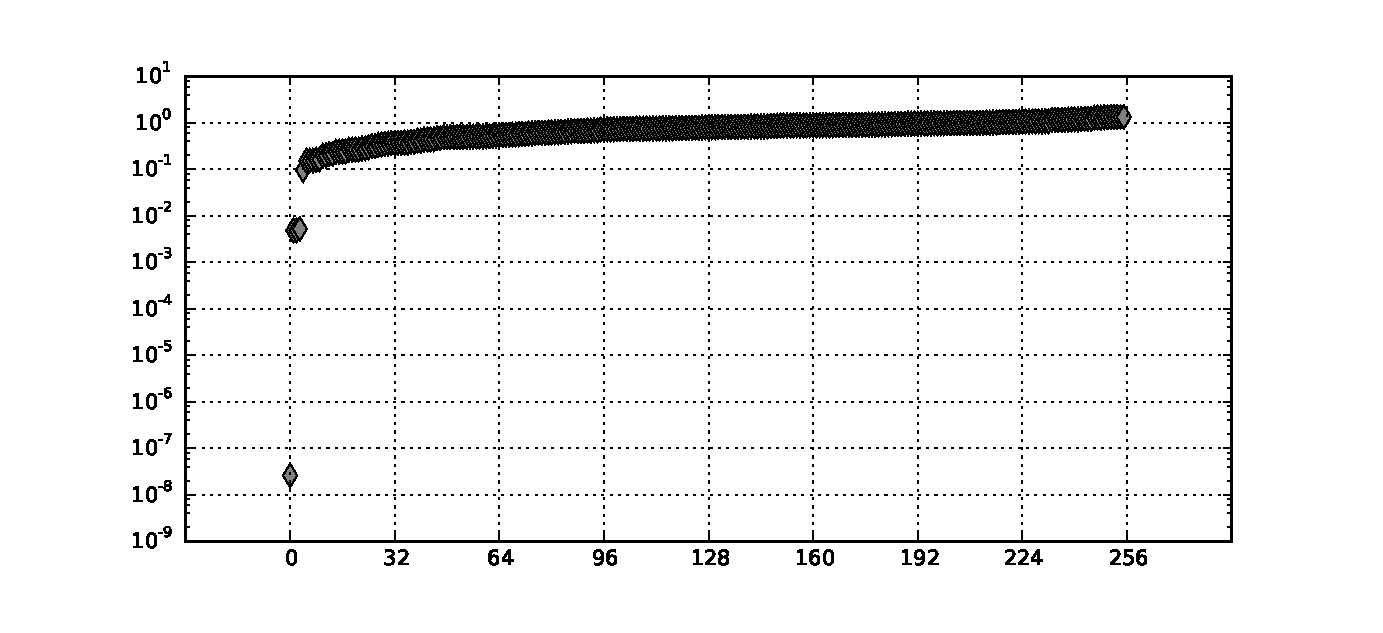
\includegraphics[width=\textwidth]{oscvalues.eps}
  \caption{The sorted magnitudes of the oscillatory parts of
    $\theta\big( \boldsymbol{h}_j - \tfrac{1}{2}\Abel_0^{\DivC}, \Omega
    \big)$ for each of the 256 half-lattice vectors
    $\boldsymbol{h}_j$. Note that the half-lattice vector resulting in
    the correct RCV produces a theta value approximately five orders of
    magnitude closer to zero than the others.}
  \label{fig:oscvalues}
\end{figure}

Even with the default numerical integration and Riemann theta accuracy
of $10^{-8}$ the choice of half-lattice vector producing the above RCV
results in a Riemann theta value that is several orders of magnitude
closer to zero than with the incorrect choices of half-lattice vector,
as shown in Figure \ref{fig:oscvalues}.

Let $\DivD$ be the divisor consisting of the three places lying above
$x=2$ each of multiplicity one. $\DivD$ is an effictive divisor of
degree $g-1 = 3$. Therefore, $\RCV(P_0) + \Abel(P_0,\DivD)$ is also a
member of the theta divisor.
\begin{ipythoninput}
D = sum(places_above_two)
W = J(AbelMap(D) + K(P0))
v = RiemannTheta.oscillatory_part(W, Omega)
print abs(v)
\end{ipythoninput}
\begin{ipythonoutput}
1.09506634962e-10
\end{ipythonoutput}
\end{example}


%%%%%%%%%%%%%%%%%%%%%%%%%%%%%%%%%%%%%%%%%%%%%%%%%%%%%%%%%%%%%%%%%%%%%%%%%%%%%%%
\section{Acknowledgements}
%%%%%%%%%%%%%%%%%%%%%%%%%%%%%%%%%%%%%%%%%%%%%%%%%%%%%%%%%%%%%%%%%%%%%%%%%%%%%%%


This work was generously supported by the National Science Foundation
under grant NSF-DMS-1008001. Any opinions, findings, and conclusions or
recommendations expressed in this material are those of the authors and
do not necessarily reflect the views of the funding sources.

%%%% REFERENCES %%%%%%%%%%%%%%%%%%%%%%%%%%%%%%%%%%%%%%%%%%%%%%%%%%%%%%%%%%%%%%%
\bibliographystyle{amsplain}
\bibliography{rcv}

\end{document}

